\documentclass[sans,mathserif,aspectratio=169, 10pt]{beamer}

\usepackage{booktabs}
\usepackage[spanish, mexico]{babel}
\selectlanguage{spanish}
\decimalpoint
\usepackage[utf8]{inputenc}
\usepackage{tikz}
\usepackage{fourier}
\newcommand{\quotes}[1]{``#1''}
\usepackage{epstopdf}
\usepackage{mathtools}
\DeclarePairedDelimiter{\ceil}{\lceil}{\rceil}
\usepackage{commath}
\usepackage{amsmath,tabularx}
\usepackage{listings}
\usepackage{xcolor}
\usepackage[edges]{forest}
\graphicspath{{Images/}}
\usepackage[mathscr]{euscript}
\newcommand{\overbar}[1]{\mkern 1.5mu\overline{\mkern-1.5mu#1\mkern-1.5mu}\mkern 1.5mu}
\newcommand*\mean[1]{\overbar{#1}}

\newcommand\Fontvi{\fontsize{9}{7.2}\selectfont}
\definecolor{foldercolor}{RGB}{124,166,198}

\tikzset{pics/folder/.style={code={%
    \node[inner sep=0pt, minimum size=#1](-foldericon){};
    \node[folder style, inner sep=0pt, minimum width=0.3*#1, minimum height=0.6*#1, above right, xshift=0.05*#1] at (-foldericon.west){};
    \node[folder style, inner sep=0pt, minimum size=#1] at (-foldericon.center){};}
    },
    pics/folder/.default={20pt},
    folder style/.style={draw=foldercolor!80!black,top color=foldercolor!40,bottom color=foldercolor}
}

\forestset{is file/.style={edge path'/.expanded={%
        ([xshift=\forestregister{folder indent}]!u.parent anchor) |- (.child anchor)},
        inner sep=1pt},
    this folder size/.style={edge path'/.expanded={%
        ([xshift=\forestregister{folder indent}]!u.parent anchor) |- (.child anchor) pic[solid]{folder=#1}}, inner xsep=0.6*#1},
    folder tree indent/.style={before computing xy={l=#1}},
    folder icons/.style={folder, this folder size=#1, folder tree indent=3*#1},
    folder icons/.default={12pt},
}

\colorlet{punct}{red!60!black}
\definecolor{background}{HTML}{EEEEEE}
\definecolor{delim}{RGB}{20,105,176}
\colorlet{numb}{magenta!60!black}

\lstdefinelanguage{json}{
    basicstyle=\normalfont\ttfamily\tiny,
    columns=flexible,
    keepspaces=true,
    frame=lines,
    backgroundcolor=\color{background}
}

\mode<presentation>

%Colors
\definecolor{steel}{RGB}{52,102,136}
\definecolor{moss}{RGB}{139,187,159}
\definecolor{burnt}{RGB}{187,102,65}
\definecolor{sandy}{RGB}{186, 168, 111}
\definecolor{RoyalBlue}{RGB}{0,35,102}
\definecolor{cream}{RGB}{254, 246, 235}
\definecolor{slate}{RGB}{82, 85, 100}
\definecolor{fall}{RGB}{194, 91, 86} % frame color
\definecolor{light}{RGB}{150, 192, 206}

%Structure
\usefonttheme{professionalfonts}
\hypersetup{colorlinks,linkcolor=fall!80,urlcolor=fall!80}
\setbeamercolor{local structure}{fg=fall}
\setbeamercolor{background canvas}{bg=cream}
\setbeamercolor{frametitle}{bg=fall,fg=cream}
\setbeamercolor{title}{fg=steel!115}
\setbeamercolor{author}{fg=fall}

\defbeamertemplate*{title page}{customized}[1][]
{\centering
  \usebeamerfont{title}\usebeamercolor[fg]{title}{\bfseries\inserttitle}\par
  \usebeamerfont{subtitle}\usebeamercolor[fg]{subtitle}\insertsubtitle\par
  \vfill
  \usebeamerfont{author}\usebeamercolor[fg]{author}\insertauthor\par
  \vfill
  \usebeamerfont{institute}\insertinstitute\par
  \usebeamerfont{date}\insertdate\par
  \usebeamercolor[fg]{titlegraphic}\inserttitlegraphic
}

% Progressbar
\usepackage{tikz}
\usetikzlibrary{calc}

\makeatletter
\def\progressbar@progressbar{} % the progress bar
\newcount\progressbar@tmpcounta% auxiliary counter
\newcount\progressbar@tmpcountb% auxiliary counter
\newdimen\progressbar@pbht %progressbar height
\newdimen\progressbar@pbwd %progressbar width
\newdimen\progressbar@tmpdim % auxiliary dimension

\progressbar@pbwd=\paperwidth
\progressbar@pbht=2pt

\def\progressbar@progressbar{%

\progressbar@tmpcounta=\insertframenumber
\progressbar@tmpcountb=\inserttotalframenumber
\progressbar@tmpdim=\progressbar@pbwd
\multiply\progressbar@tmpdim by \progressbar@tmpcounta
\divide\progressbar@tmpdim by \progressbar@tmpcountb

  \begin{tikzpicture}[very thin]

  \shade[draw=steel!115,top color=steel,bottom color=steel,middle color=steel!115] %
    (0pt, 0pt) rectangle ++ (\progressbar@tmpdim, \progressbar@pbht);

  \end{tikzpicture}%
 }

\addtobeamertemplate{frametitle}{}
{%
  \vspace*{-16pt}
  \begin{beamercolorbox}[wd=\paperwidth,ht=1pt,dp=1pt]{}%
    \progressbar@progressbar%
  \end{beamercolorbox}%
}%
\makeatother

%Title
\title{Subgroup Resonance Calculation Methodology Improvements}
\subtitle{a holistic approach}
\author[Guillermo Ibarra]{Guillermo Ibarra}
\date{Nuclear Engineering Research Seminar, May 19th, 2020}

\definecolor{keywords}{RGB}{255,0,90}
\definecolor{comments}{RGB}{0,0,113}
\definecolor{red}{RGB}{160,0,0}
\definecolor{green}{RGB}{0,150,0}

\setbeamercovered{transparent}
\setbeamercovered{%
  again covered={\opaqueness<1->{40}}}
\beamertemplatenavigationsymbolsempty

\begin{document}

%slide
\begin{frame}
\titlepage
\end{frame}

%slide
\begin{frame}{Resonance Calculations\footnote[frame,1]{D. Knott y A. Yamamoto, “Lattice physics computations,” en Handbook of Nuclear Engineering (D. Cacuci,
ed.), vol. II Reactor Design, pp. 913–1239, Springer Science+Business Media, 2010.}}{in context}
\centering
\fcolorbox{fall}{white}{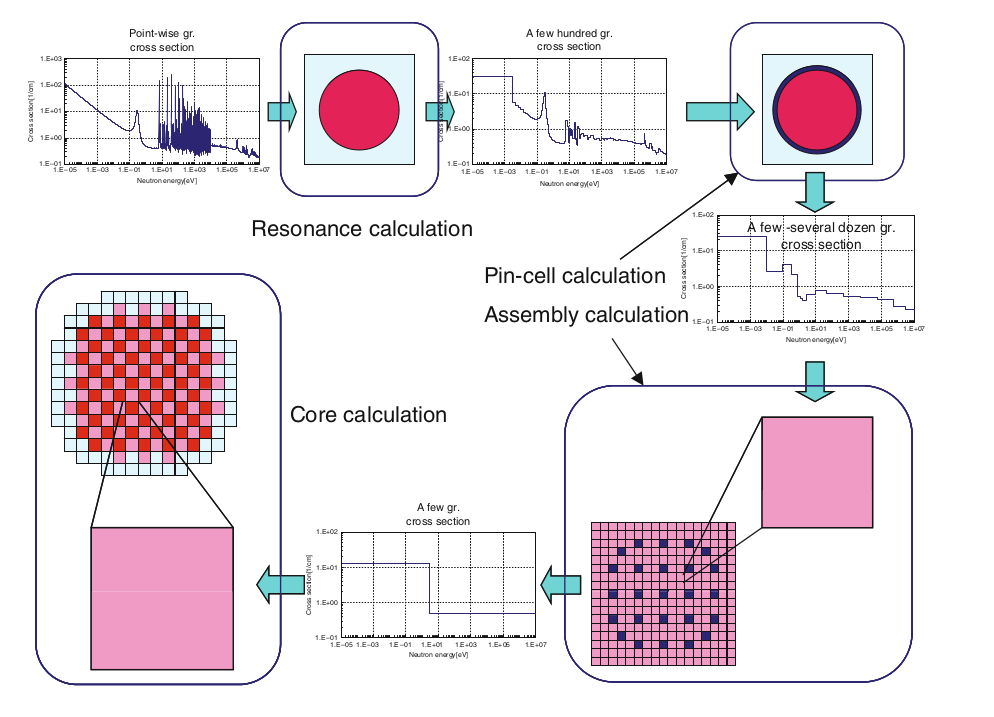
\includegraphics[width=0.60\linewidth]{generalCalculation.png}}
\end{frame}

%slide
\begin{frame}{Energetic Resonance\footnote[frame,1]{D. Knott y A. Yamamoto, “Lattice physics computations,” en Handbook of Nuclear Engineering (D. Cacuci,
ed.), vol. II Reactor Design, pp. 913–1239, Springer Science+Business Media, 2010.}}
\centering
\fcolorbox{fall}{white}{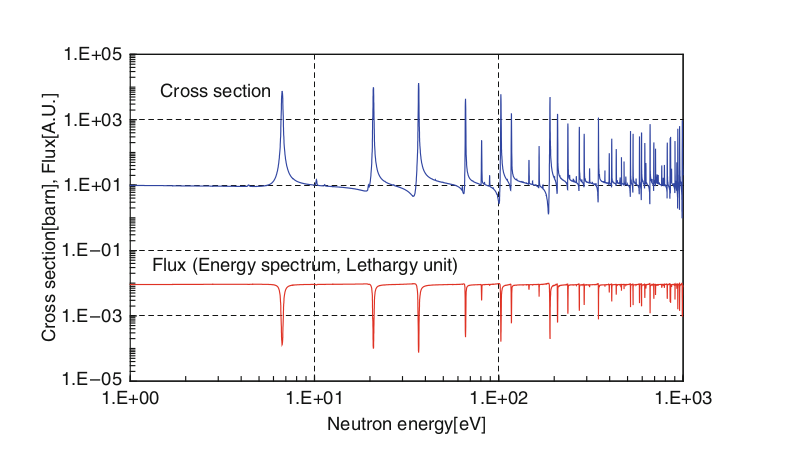
\includegraphics[width=0.60\linewidth]{spectrum.png}}
\end{frame}

%slide
\begin{frame}{Spatial Resonance\footnote[frame,1]{D. Knott y A. Yamamoto, “Lattice physics computations,” en Handbook of Nuclear Engineering (D. Cacuci,
ed.), vol. II Reactor Design, pp. 913–1239, Springer Science+Business Media, 2010.}}
\centering
\fcolorbox{fall}{white}{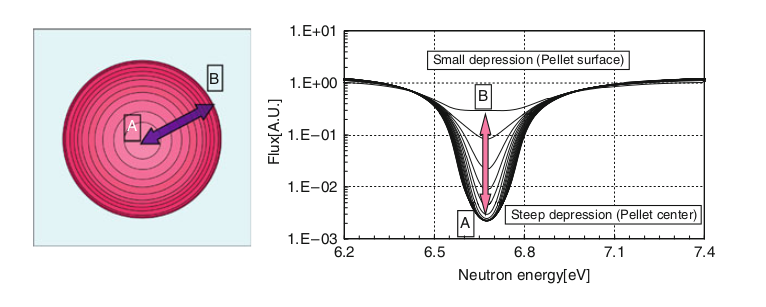
\includegraphics[width=0.65\linewidth]{spatial.png}}
\end{frame}

%slide
\begin{frame}{General Overview}{resonance methods}
\begin{itemize}
\item<1> Equivalence 
\item<2> Ultrafine
\item<3> Subgroup
\end{itemize}
\end{frame}

%slide
\begin{frame}{Subgroup Method}
\centering
\fcolorbox{fall}{white}{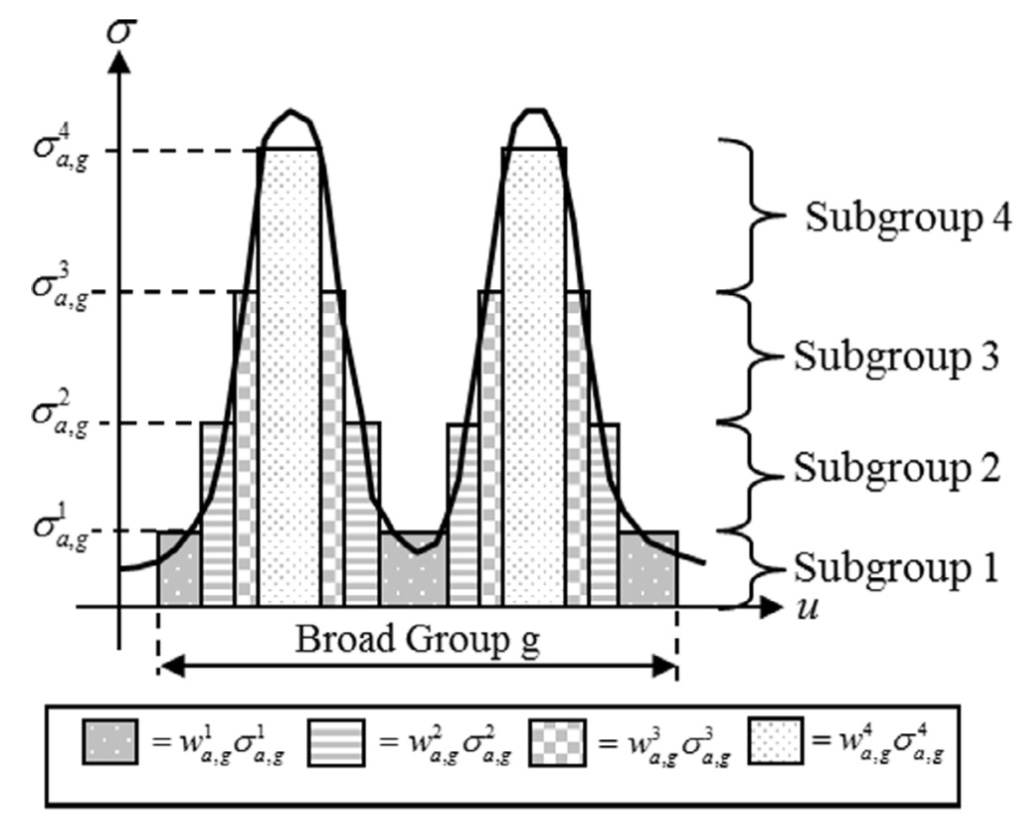
\includegraphics[width=0.65\linewidth]{subgroup.jpeg}}
\end{frame}

%slide
\begin{frame}{General Overview}{general concerns [Liu and Martin, 2017]}
\begin{itemize}
\item<1> spatial self-shielding effects 
\item<2> resonance interference
\item<3> non-uniform temperature effects
\item<4-> self-shielding of clad isotopes
\end{itemize}
\end{frame}

%slide
\begin{frame}{Spatial Self-Shielding Effects [Liu and Martin, 2017]}
\begin{minipage}{0.48\linewidth}
\centering
\fcolorbox{fall}{white}{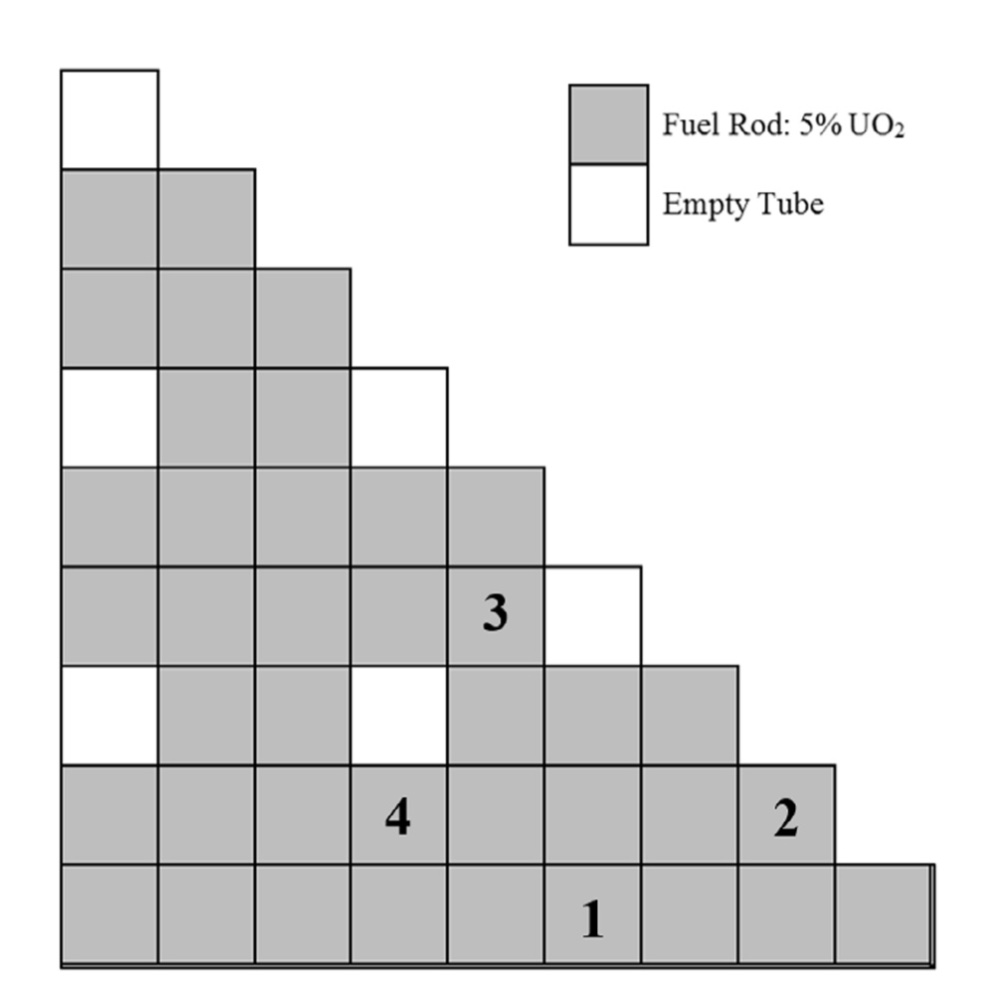
\includegraphics[width=0.85\linewidth]{pwrAssembly.jpeg}}
\end{minipage}\hfill
\begin{minipage}{0.48\linewidth}
\centering
\fcolorbox{fall}{white}{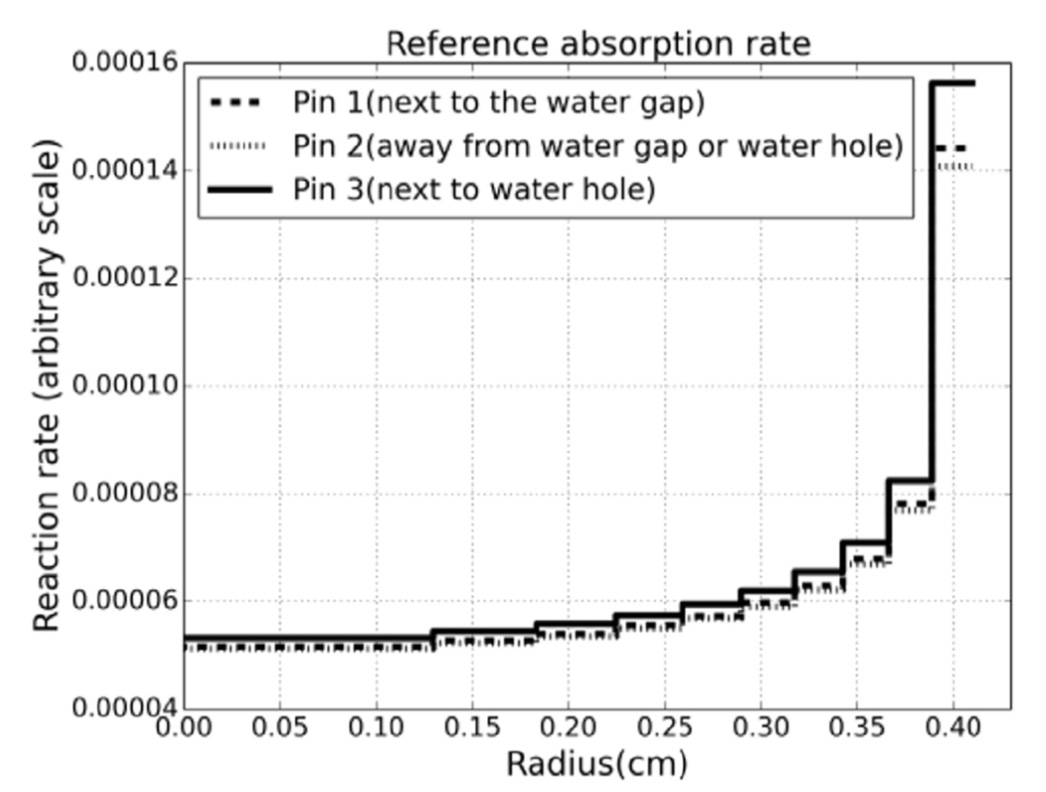
\includegraphics[width=0.9\linewidth]{pwrSpatial.jpeg}}
\end{minipage}
\end{frame}

%slide
\begin{frame}{Interference Effects [Soppera et al. 2014]}
\centering
\fcolorbox{fall}{white}{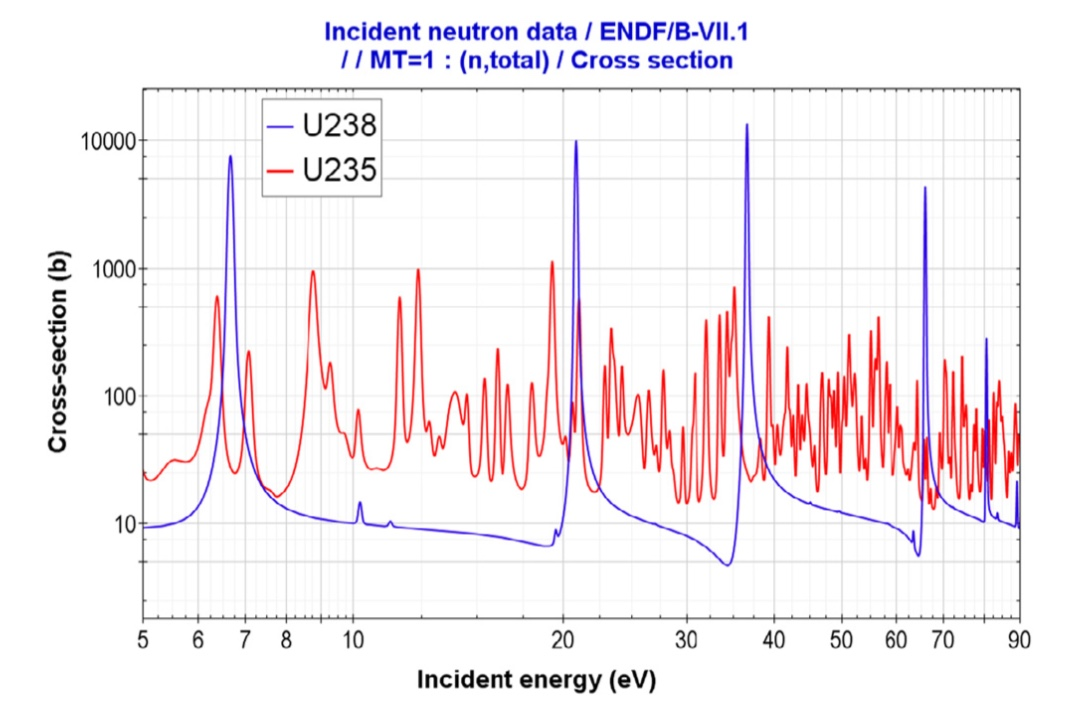
\includegraphics[width=0.65\linewidth]{interference.jpeg}}
\end{frame}

%slide
\begin{frame}{Resonance Interference Factors (RIF)}
\begin{itemize}
\item<1> Tabular values [Choi et al. 2015]
\item<2> Subgroup weights [Joo et al. 2009]
\end{itemize}
\end{frame}

%slide
\begin{frame}{Primary Objective}
\large 
Develop a self-shielding methodology for a 2D heterogenous system, capable of performing high fidelity whole core direct transport calculations. Such that within pin effects are considered, these include multi-region depletion and non uniform temperature distribution. 
\end{frame}

%slide
\begin{frame}{Proposed Roadmap}
\begin{itemize}
\item<1> Gemma conditioning.
\item<2> WIMS structure library adoption and resonance models.
\item<3> New library generation with NJOY.
\item<4> Adoption of a \emph{better} equivalence method [Choi et al. 2017].
\item<5> Application of a \emph{better} subgroup method [Lu et al. 2018] and ESSM-X [Liu et al. 2015] 
\end{itemize}
\end{frame}

%slide
\begin{frame}
\centering
\Huge
Thanks! \\
Questions?
\end{frame}


\end{document}
